\documentclass[usenames,dvipsnames]{beamer}
\usepackage[utf8]{inputenc}
\usepackage[T1]{fontenc}
\usepackage[french]{babel}
\usepackage{xcolor}
\usepackage{pifont}
\usetheme{Singapore} %Boadilla | Bergen | Madrid | Antibes | Hannover | Singapore | Warsaw

\newcommand{\cmark}{\ding{51}}
\newcommand{\xmark}{\ding{55}}
%----------------------------------------------------------------------------------------
%   TITLE INFORMATION
%----------------------------------------------------------------------------------------
\title{CourtCircuit}
\subtitle{HLSE602 -- Projet CMI Annuel}
\author{B. Rima \and O. Farajallah \and W. Soussi}
\institute[UM]{L3 CMI Informatique}
\date{\today}

\begin{document}
%----------------------------------------------------------------------------------------
%   TITLE FRAME
%----------------------------------------------------------------------------------------
\begin{frame}
\titlepage
\end{frame}
%----------------------------------------------------------------------------------------
%   OUTLINE
%----------------------------------------------------------------------------------------
\begin{frame}{Sommaire}
\tableofcontents
\end{frame}
%----------------------------------------------------------------------------------------
%   INTRODUCTION
%----------------------------------------------------------------------------------------
\section{Introduction}
\begin{frame}{Contexte du projet}{Introduction}
  \begin{description}
    \item [Projet CMI :] Module d'un projet annuel pour l'année 2017--2018 dans le cadre du \textbf{CMI Informatique}
    \item [Responsable CMI Informatique :] Mme Anne-Elisabeth Baert
    \item [Encadrant du projet :] M. Eric Bourreau
    \item [Lieux de travail :] La \textbf{FDS} et le \textbf{LIRMM}
  \end{description}
\end{frame}

%----------------------------------------------------------------------------------------
%   RAPPELS
%----------------------------------------------------------------------------------------
\section{Rappels}
%----------------------------------------------------------------------------------------
%   PROBLÉMATIQUE
%----------------------------------------------------------------------------------------
\subsection{Problématique}
\begin{frame}{Rappels}{Problématique}
\begin{columns}[onlytextwidth, T]
  \column{50mm}
    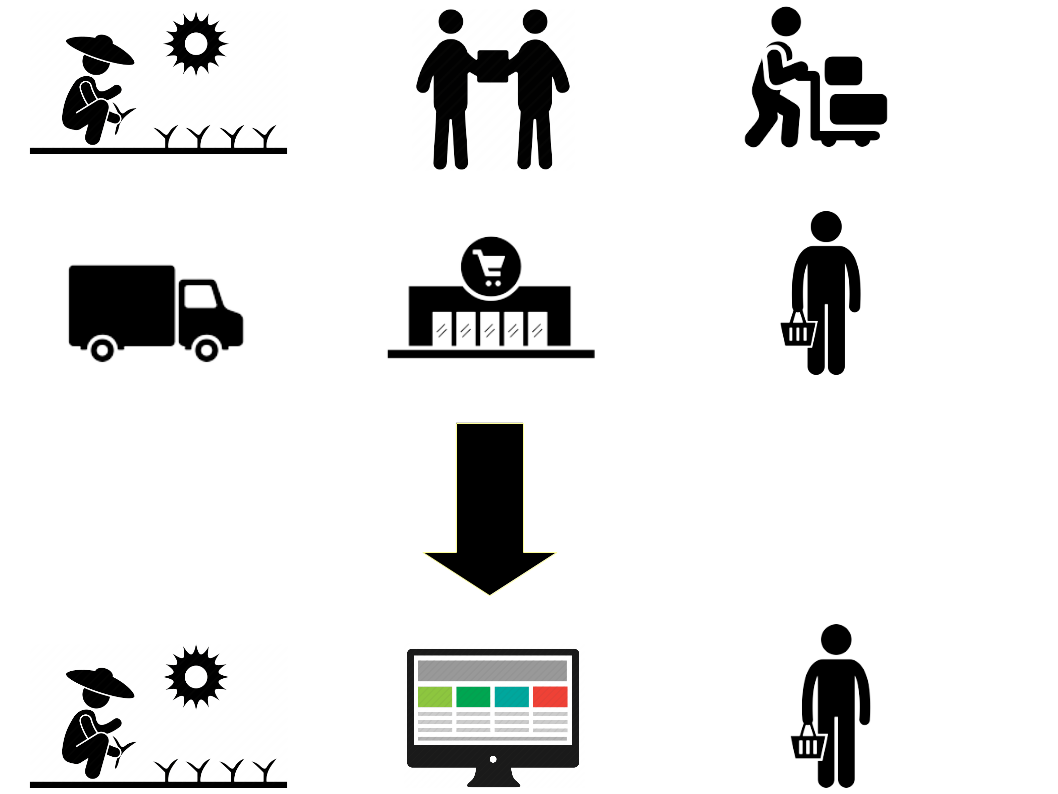
\includegraphics[scale=0.19]{images/chain_production.png}

  \column{\dimexpr\linewidth-35mm-4mm}
    \begin{block}{Consommateurs :}
    Acheter des produits frais et minimiser \\les étapes de processing.
    \end{block}

    \begin{block}{Producteurs :}
    Maîtriser le prix de vente et \\les débouchés de leurs productions en \\se libérant des intermédiaires de distribution.
    \end{block}
\end{columns}
\end{frame}
%----------------------------------------------------------------------------------------
%   SOLUTION PROPOSÉE : COURTCIRCUIT
%----------------------------------------------------------------------------------------
\subsection{Solution proposée : \texttt{CourtCircuit}}
\begin{frame}{Rappels}{Solution proposée : \texttt{CourtCircuit}}
  \begin{block}{Site web \textit{e-commerce}}
  Une interface directe entre \textbf{consommateurs} et \textbf{fournisseurs}.
  \end{block}

  \begin{block}{Ruche}
  Un regroupement de plusieurs \textbf{fournisseurs} d'une région, \textbf{sans guide explicite} préfixé par le site, associé à plusieurs points de collecte.
  \end{block}

  \begin{block}{Vision Décentralisée et Autonome}
  \begin{itemize}
    \item l'ensemble des ruches ne répond à \textbf{aucune entité centrale}.
    \item chaque ruche s'occupe de ses propres besoins et de leur gestion sans besoin d'un intermédiaire et d'une hiérarchie à respecter.
  \end{itemize}
  \end{block}
\end{frame}
%----------------------------------------------------------------------------------------
%   OUTILS DE CONCEPTION
%----------------------------------------------------------------------------------------
\subsection{Outils de conception}
\begin{frame}{Rappels}{Outils de conception}
  \begin{enumerate}
    \item \textit{User Stories} (outil de conception agile)
    \item Diagrammes de cas d'usage
    \item Modèle EA
    \item Schéma de base de données
    \item \textit{Storyboard}
  \end{enumerate}
\end{frame}
%----------------------------------------------------------------------------------------
%   IMPLÉMENTATION
%----------------------------------------------------------------------------------------
\section{Implémentation}
%----------------------------------------------------------------------------------------
%   APPLICATION WEB MONOPAGE
%----------------------------------------------------------------------------------------
\subsection{Application web monopage}
\begin{frame}{Application web monopage (Introduction)}{Implémentation}
  \begin{figure}[!ht]
    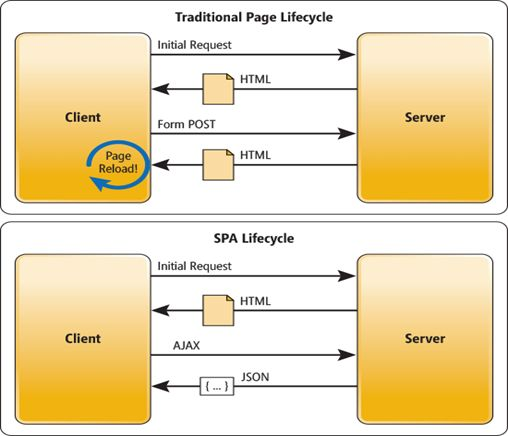
\includegraphics[scale=0.5]{images/SPAvsTRADITIONAL.jpg}
  \end{figure}
\end{frame}

\begin{frame}{Application web monopage (Avantages)}{Implémentation}
  \begin{itemize}
    \item chargement plus rapide de la page.
    \item séparation des tâches de contrôle et de vue $\rightarrow$ meilleure implémentation des contraintes du \textit{design pattern} \textbf{MVC}.
    \item facilité de déploiement.
  \end{itemize}
\end{frame}
%----------------------------------------------------------------------------------------
%   OUTILS D'IMPLÉMENTATION
%----------------------------------------------------------------------------------------
\subsection{Outils d'implémentation}
\begin{frame}{Outils d'implémentation}{Implémentation}
  \begin{figure}[!ht]
    \centering
    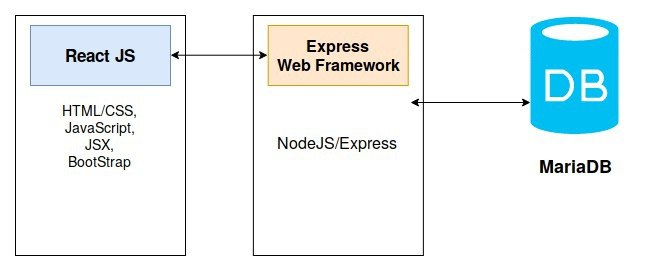
\includegraphics[scale=0.3]{images/website_architecture.jpeg}
  \end{figure}

  \begin{description}
    \item [\textit{Front-end} :] React.js, JSX, Bootstrap
    \item [\textit{Back-end} :] Node.js, Express.js
    \item [Base de données :] MariaDB
  \end{description}
\end{frame}
%----------------------------------------------------------------------------------------
%   FRONT-END
%----------------------------------------------------------------------------------------
\subsection{\protect\textit{Front-end}}
%----------------------------------------------------------------------------------------
%   REACT
%----------------------------------------------------------------------------------------
\begin{frame}{\textit{React}}{Front-end}

\end{frame}
%----------------------------------------------------------------------------------------
%   BOOTSTRAP ET FONT-AWESOME
%----------------------------------------------------------------------------------------
\begin{frame}{\textit{Bootstrap et Font-Awesome}}{Front-end}
  \begin{figure}[!ht]
    
\includegraphics[scale=0.065]{images/bootstrapLogo.jpg}
    \hfill
    
\includegraphics[scale=0.15]{images/font_awesome.png}
  \end{figure}

  \begin{itemize}
    \item réalisation de pages \textbf{responsives}.
    \item personnalisation de la mise en forme des pages à travers des \textbf{classes CSS} prédéfinies.
    \item icônes modifiables dynamiquement.
  \end{itemize}

  \begin{figure}[!ht]
    
\includegraphics[scale=0.2]{images/header_navbar_component.png}
    \caption{Entête du site faite avec la classe \textit{Navbar} de \textbf{Bootstrap} avec des icônes \textbf{Font-awesome}}
  \end{figure}
\end{frame}
%----------------------------------------------------------------------------------------
%   BACK-END
%----------------------------------------------------------------------------------------
\subsection{\protect\textit{Back-end}}
%----------------------------------------------------------------------------------------
%   NODE.JS
%----------------------------------------------------------------------------------------
\begin{frame}{\textit{Node.js} (Introduction)}{Back-end}
  \begin{figure}[!ht]
    
\includegraphics[scale=0.03]{images/nodejs_icon.png}
  \end{figure}

  \begin{itemize}
    \item environnement d'exécution \textbf{JavaScript} côté serveur utilisant le moteur \textbf{JavaScript V8} de \textit{Google Chrome}.
    \item gratuit et \textit{open-source}.
    \item modélisation événementielle, monothread et non-bloquante.
    \item architecture modulaire.
    \item gestionnaire de paquets \textbf{NPM} (\textit{Node Package Manager}) $\rightarrow$ facilité d'usage et d'extensibilité.
  \end{itemize}
\end{frame}

\begin{frame}{\textit{Node.js} (Raisons du choix)}{Back-end}
  \begin{itemize}
    \item écrire du code \textbf{JavaScript} du côté serveur $\rightarrow$ un seul langage pour les côtés client et serveur.
    \item modélisation événementielle, monothread et non-bloquante $\rightarrow$ performance fluide et gestion efficace d'un ensemble important de données.
    \item ensemble important de modules utilitaires facilement téléchargeable via \textbf{NPM}.
  \end{itemize}
\end{frame}

\begin{frame}{\textit{Node.js} (Utilisation)}{Back-end}
  \begin{itemize}
    \item création d'une \textbf{API} factorisée, non redondante et facilement lisible (\textit{Client, Fournisseur, Produit, $\dots$}) permettant d'interfacer avec la base de données.
    \item héberger \textbf{Express}.
  \end{itemize}
\end{frame}
%----------------------------------------------------------------------------------------
%   EXPRESS
%----------------------------------------------------------------------------------------
\begin{frame}{\textit{Express} (Introduction)}{Back-end}
  \begin{figure}[!ht]
    \centering
    
\includegraphics[scale=0.2]{images/express_icon.png}
  \end{figure}

  \begin{itemize}
    \item framework web minimaliste pour \textbf{Node.js}.
    \item gratuit et \textit{open-source}.
    \item utilisation de \textit{middleware}.
    \item gestion des routes \textbf{REST} (\textit{Representational State Transfer}) et des formulaires en s'appuyant sur des concepts du \textit{design pattern} \textbf{MVC}.
    \item moteurs de templates (\textit{EJS (Embedded JavaScript), Pug, Handlebars, $\dots$}).
  \end{itemize}
\end{frame}

\begin{frame}{\textit{Express} (Raisons du choix et utilisation)}{Back-end}
  \begin{itemize}
    \item framework web \textit{de-facto} pour \textbf{Node.js}.
    \item réduire la verbosité du code \textbf{Node.js} natif pour la création du serveur \textbf{HTTP}.
    \item utilisation de \textit{middleware} pour le traitement des requêtes clients.
    \item gestion des routes \textbf{REST} pour les opérations \textbf{CRUD}.
  \end{itemize}
\end{frame}
%----------------------------------------------------------------------------------------
%   MARIADB
%----------------------------------------------------------------------------------------
\begin{frame}{\textit{MariaDB} (Introduction)}{Back-end}
  \begin{figure}[!ht]
    \centering
    
\includegraphics[scale=0.35]{images/mariadb_icon.png}
  \end{figure}

  \begin{itemize}
    \item \textbf{SGBD} relationnel.
    \item gratuit et \textit{open-source}.
    \item assure l'interopérabilité avec \textbf{MySQL}.
    \item introduit par les créateurs de \textbf{MySQL} suite à l'achat de ce dernier par \textbf{Oracle}.
  \end{itemize}
\end{frame}

\begin{frame}{\textit{MariaDB} (Raisons du choix et utilisation)}{Back-end}
  \begin{itemize}
    \item fork communautaire de \textbf{MySQL} mis à jour plus souvent que ce dernier.
    \item \textbf{modèle EA} déjà traduit en \textbf{modèle relationnel} depuis la phase de conception du projet $\rightarrow$ mise en \oe{}uvre directe.
    \item mise en place d'un système de validation des données dans le cadre d'une politique de sécurité en trois couches (\textit{client, serveur, base de données}) $\rightarrow$ assurer l'intégrité des données stockées.
    \item le serveur de la faculté qui nous a été attribué pour le déploiement hébérge bien \textbf{MySQL} $\rightarrow$ possibilité d'utiliser \textbf{MariaDB}.
  \end{itemize}
\end{frame}
%----------------------------------------------------------------------------------------
%   RÉSULTATS
%----------------------------------------------------------------------------------------
\section{Résultats}
%----------------------------------------------------------------------------------------
%   BILAN
%----------------------------------------------------------------------------------------
\subsection{Bilan}
\begin{frame}{Bilan}{Résultats}
\begin{table}[!ht]
  \centering
  \begin{tabular}{|l|c|}
  \hline
  Base de données conçue et testée & \cmark\\
  \hline
  Composants de base de l'interface graphique & \cmark\\
  \hline
  Connexion du client au serveur & \cmark\\
  \hline
  Connexion du serveur à la base de données & \cmark\\
  \hline
  Gestion des routes entre le serveur et le client & \xmark\\
  \hline
  Test du comportement dynamique des composants & \xmark\\
  \hline
  Déploiement en ligne & \xmark\\
  \hline
  \end{tabular}
  \caption{Bilan des résultats}
\end{table}
\end{frame}
%----------------------------------------------------------------------------------------
%   DIFFICULTÉS SURVENUES
%----------------------------------------------------------------------------------------
\subsection{Difficultés survenues}
\begin{frame}{Difficultés survenues}{Résultats}
  \begin{itemize}
    \item nouveaux concepts et outils d'implémentation nécessitant un temps d'apprentissage considérable.
    \item temps d'apprentissage considérable $\rightarrow$ adoption d'une méthodologie agile de développement de plus en plus compliqué.
    \item temps dédié à l'implémentation insuffisant.
    \item problèmes liés au serveur d'hébergement.
  \end{itemize}
\end{frame}
%----------------------------------------------------------------------------------------
%   CONCLUSION
%----------------------------------------------------------------------------------------
\section{Conclusion}
%----------------------------------------------------------------------------------------
%   APPORTS PERSONNELS DU PROJET
%----------------------------------------------------------------------------------------
\subsection{Apports personnels du projet}
\begin{frame}{Apports personnels du projet}{Conclusion}
  \begin{itemize}
    \item Apports personnels = difficultés survenues.
    \item Apprentissage d'outils \textit{front-end} et \textit{back-end} récents et en pleine évolution.
    \item Appréciation plus profonde du langage \textbf{JavaScript}.
  \end{itemize}
\end{frame}
%----------------------------------------------------------------------------------------
%   PERSPECTIVES
%----------------------------------------------------------------------------------------
\subsection{Perspectives}
\begin{frame}{Perspectives}{Conclusion}
  \begin{itemize}
    \item Continuation du projet au niveau personnel.
    \item Récolte de \textit{feedback} des utilisateurs potentiels.
    \item Mise en place et optimisation de la logistique.
    \item Implémentation de fonctionnalités supplémentaires (paiement en ligne, commandes retardées, portefeuille virtuel, $\dots$).
    \item Internationalisation.
 \end{itemize}
\end{frame}
\end{document}
